\chapter{Visualisierung der Schmerzbewertung}
\label{sec:visualisation}

In \autoref{sec:deduction} wurde das Konzept zur Schmerzbewertung auf Basis akustischer Signale vorgestellt. Wird dieses Konzept zur kontinuierlichen Überwachung von Neugeborenen eingesetzt, fällt eine große Menge an Auswertungsergebnissen an. Daher ist es wünschenswert, die Ergebnisse der automatisierten Schmerzbewertung übersichtlich zu visualisieren. In \autoref{sec:vizConecept} wird das Konzept der Visualisierung vorgestellt. Die Visualisierung fokussiet die Visualisierung des Scores, der im Zuge der Schmerzbewertung für den Schmerzindikator \emph{Weinen} auf Basis der Audiosignals vergeben wird. \autoref{sec:vizResults} fasst die Visualisierungsergebnisse zusammen.

\section{Visualierungskonzept}
\label{sec:vizConecept}

Das Visualisierungskonzept wird anhand eines 220 Sekunden langen Audioaufnahme eines weinenden Babys erläutert. Das Signal wird in \autoref{img:visualisation_example_01} oben gezeigt. Die stimmhaften Signalbereiche werden Schwarz dargestellt, das Hintergrundrauschen grau. Das Signal wurde nach der in \autoref{sec:segmenting} beschriebenen Methode segmentiert mit $t_{s} = \SI{10}{\second}$. Die Schreigeräusche wurden so zu zwei Segmenten $cs_1$ und $cs_2$ zusammengefasst, welche in der Abbildung ebenfalls oben hervorgehoben werden.

\begin{figure}[h]
	\centering
	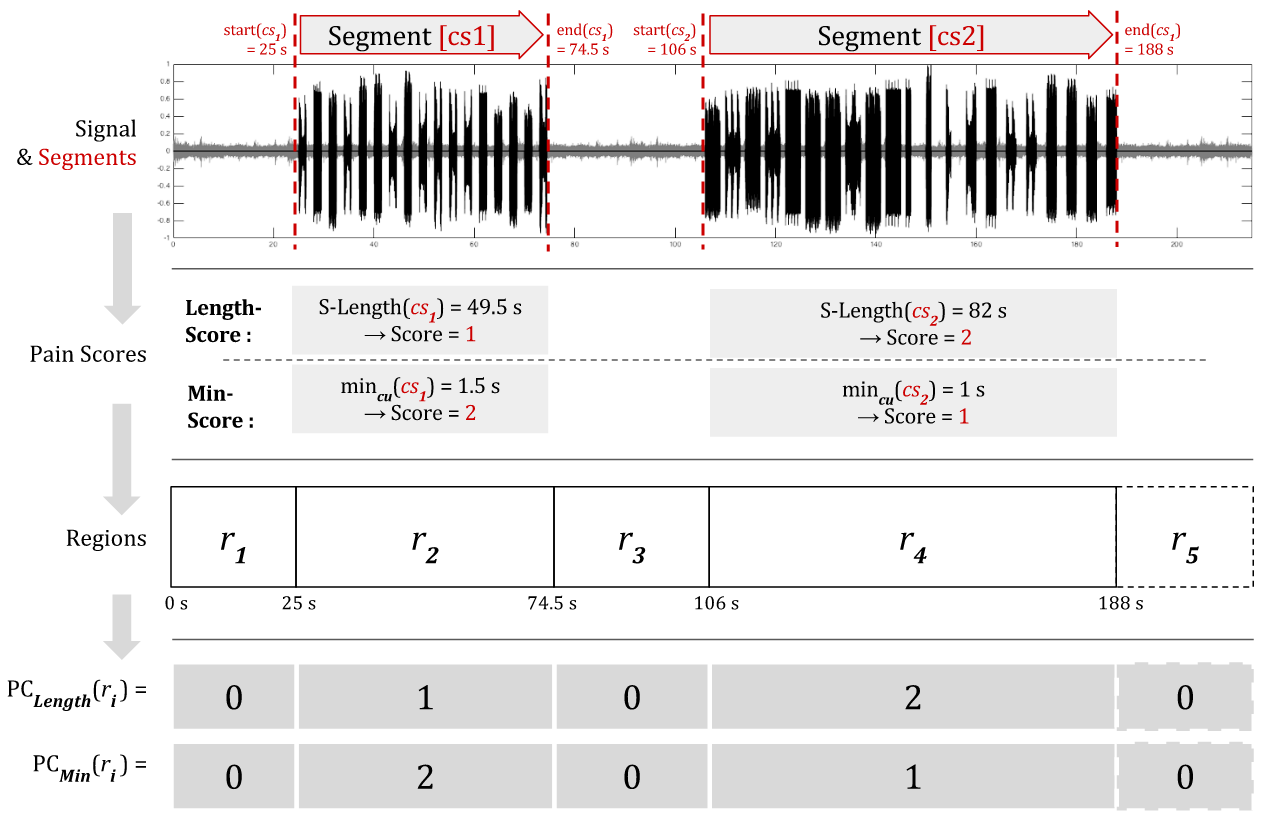
\includegraphics[width=1\textwidth]{bilder/visualisation_example_02.png}
	\caption[Einteilung eines Signals in Regionen zur Vorbereitung der Visualisierung]{Oben: Ein Beispielsignal mit zwei Segmenten. Darunter: Schmerz-Scores, die für die beiden Segmente auf Basis der beiden fiktiven Schmerz-Scales aus \autoref{tab:fictional_painscales_viz} mit Hilfe der Hypothesen aus \autoref{eq:ps_length_hypothesis} und \autoref{eq:min_length_hypothesis} berechnet wurden. Darunter: Schematische Darstellung des Signals durch Regionen. Unten: Schmerz-Scores der Regionen.}
	\label{img:visualisation_example_01}
\end{figure}

Die Schmerzbewertung wird auf Basis von zwei fiktiven Schmerz-Scales durchgeführt. Die Bewertung des Schmerzindikators \emph{Weinen} wird in Tabelle \ref{tab:fictional_painscales_viz} definiert. Die \glqq Length-Scale\grqq{} bewertet den Schmerzgrad nach der Länge des Weinens und definiert einen maximalen Score on 2, die \glqq Min-Scale\grqq{} bewertet die Qualität des Weinens und definiert einen maximalen Score von 3, da die Schmerz-Scale 3 Scores definiert. Es wird zunächst davon ausgegangen, dass es sich bei den Schmerz-Scales um monomdale Schmerz-Scales handelt, die nur das Weinen bei der Schmerzbewertung betrachten und keine weiteren Schmerzindikatoren mit einbeziehen. Das heißt, dass der für das Weinen vergebene Score einem Schmerz-Score entspricht.

\begin{table}[h]
\centering
\caption{Bewertung des Weinens von zwei fiktive Schmerz-Scales}
\label{tab:fictional_painscales_viz}
\begin{tabular}{@{}lll@{}}
\toprule
Score       & \glqq Length-Scale\grqq  & \glqq Min-Scale\grqq        \\ \midrule
0 & kein Weinen   & Lachen           \\
1 & kurzes Weinen & leichtes Weinen  \\
2 & langes Weinen & mittleres Weinen \\
3 & -             & starkes weinen   \\ \bottomrule
\end{tabular}
\end{table}

Mit Hilfe des in \autoref{sec:overviewPainRegression} vorgestellten Vorgehen wurden Hypothesen zur Schmerzbewertung für die Schmerz-Scales definiert, um die Schmerzbewertung anhand objektiv messbarer Kriterien durchführen zu können. \autoref{eq:ps_length_hypothesis} definiert die Hypothese $PC_{Length}$ für die \emph{Length-Scale}. Die maßgebende Eigenschaft dieser Scale ist die \emph{Länge des Schrei-Segmentes}, welche in \autoref{eq:segment_length} definiert wurde.

\begin{equation}
PC_{Length}(cs) = \begin{cases}
 1 \quad ,  \text{wenn } \text{S-Length}(cs) \leq \SI{1}{\minute} \\
 2 \quad ,  \text{wenn } \text{S-Length}(cs) > \SI{1}{\minute}
 \end{cases}	
 \label{eq:ps_length_hypothesis}
\end{equation}

\autoref{eq:min_length_hypothesis} definiert die Hypothese $PC_{Min}$ für die \emph{Min-Scale} zur Schmerzbewertung nach der \glqq Min-Scale\grqq. Die maßgebende Eigenschaft ist bei dieser Scale die \emph{geringste Länge einer Schreieinheit in einem Schrei-Segment}, welche in \autoref{eq:featuresOfCryUnits} definiert wurde.

\begin{equation}
PC_{Min}(cs) = \begin{cases}
 0 \quad ,  \text{wenn } min_{cu}(cs) < \SI{0.3}{\second}\\
 1 \quad ,  \text{wenn } \SI{0.3}{\second} \leq min_{cu}(cs) \leq \SI{1}{\second}\\
 2 \quad ,  \text{wenn } \SI{1}{\second} < min_{cu}(cs) \leq \SI{2}{\second} \\
 3 \quad , \text{sonst }
 \end{cases}	
 \label{eq:min_length_hypothesis}
\end{equation}

Mit Hilfe dieser Hypothese wurde die Schmerzbewertung für das Beispielsignal in \autoref{img:visualisation_example_01} vorgenommen. Es wurden dabei keine Aktualisierungsfrequenzen oder Beobachtungszeiträume genutzt. Das erste Schrei-Segment erhält nach der \emph{Length-Scale} einen Schmerz-Score von 1 und nach der \emph{Min-Scale} einen Schmerz-Score von 2. Das zweite Schrei-Segment erhält nach der \emph{Length-Scale} einen Schmerz-Score von 2 und nach der\emph{Min-Scale} einen Schmerz-Score von 1.

Die grundlegende Idee der Visualisierung ist, den zeitlichen Verlauf des Signals schematisch als einen \emph{Balken} darzustellen. Dieser Balken repräsentiert die Zeitachse des Signals und wird in \emph{Regionen} eingeteilt. Eine Region $r$ beinhaltet entweder ein Schrei-Segment oder den Stillebereich zwischen zwei Schrei-Segmenten. Reihenfolge und Länge der Regionen entspricht der der Segmente. Für das Beispielsignal in Abbildung \ref{img:visualisation_example_01} ergebnen sich fünf Regionen $r_{1} , \ldots , r_5 $, wobei die Region $r_2$ und $r_4$ jeweils ein Schrei-Segment enthalten. Wird angenommen, dass dieses Beispielsignal noch nicht beendet wurde und weiter kontinuierlich eingelesen wird, ist die letzte Region noch nicht abgeschlossen.

Jeder Region wird ein Schmerz-Score zugewiesen. Enthält die Region ein Segment, so wird der Score des Segmentes für die Region übernommen. Regionen ohne Segment erhalten, unabhängig von der verwendeten Schmerz-Scale, einen Score von 0, wie \autoref{eq:region_score} definiert. Es wird davon ausgegangen, dass ein Score von 0 bei jeder Schmerz-Scale den Zustand \glqq kein Schmerz\grqq{} codiert, was zumindest bei allen in \autoref{tab:painscores} vorgestellten Schmerz-Scales der Fall ist. Diese Annahme stützt sich ebenfalls auf die Argumentation aus \autoref{sec:segmenting}. Abbildung \ref{img:visualisation_example_01} visualisiert im untersten Bereich diese Zuweisung von Scores zu den Regionen.

\begin{equation}
PC_{\text{Scale}}(r) = \begin{cases}
 0 \qquad \qquad \;,  \text{wenn } r  \text{ kein Schrei-Segment beinhaltet} \\
 PS_{\text{Scale}}(cs) \;, \text{wenn } r  \text{ ein Schrei-Segment beinhaltet}
 \end{cases}	
 \label{eq:region_score}
\end{equation}

Das Ziel ist nun, jede Region mit einer Farbe einzufärben, die den entsprechenden Score anzeigt. Dazu wird für jede Schmerz-Scale eine Funktion $F_{Scale}:S_{Scale} \mapsto P_{Scale}$ benötigt, welche einen Schmerz-Score auf eine Farbe abbildet. Eine Abbildungsfunktion $F_{Scale}$ wird in diesem Zusammenhang als \emph{Farbschema} bezeichnet und der Funktionsbereich $P_{Scale}$ als \emph{Farbpalette}. Ein Farbschema soll die folgenden Kriterien erfüllen:

\begin{description}
\item[Injektivität] Jeder Score einer Scale soll anhand seiner Farbe eindeutig erkennbar sein. Dementsprechend soll gelten: $|S_{Scale}| \leq |P_{Scale}|$.
\item[Intuitive Farbsemantik durch Ampelschema] Ein Farbschema soll eine intuitive Zuordnung zwischen der Höhe des Score und der jeweiligen Farbe ermöglichen. In dieser Arbeit wurde sich für ein Ampelschema entschieden. Das heißt, dass für eine Schmerz-Scale der jeweils niedrigste Score \glqq grün\grqq{}, der höchste Score \glqq rot\grqq{} und ein \glqq mittlerer\grqq{} Score als \glqq leicht rötliches gelb\grqq{} dargestellt wird. Definiert eine Schmerz-Scale einen maximalen Score von 2 bezüglich des Weinens, so wie beispielsweise das FLACC-System, so ergibt sich die Abbildung $F_{FLACC}(0) = $ \emph{grün}, $F_{FLACC}(1) = gelb$, $F_{FLACC}(2) = rot$ (siehe \autoref{tab:painscores}). Definiert eine Schmerz-Scale mehr Scores, so wie beispielsweise das MBPS mit ingesamt fünf möglichen Scores, so müssen geeignete Zwischenfarben definiert werden. Daraus folgt, dass zwei Schmerz-Scales, deren Menge an Scores gleich groß ist, das selbe Farbschema verwenden.
\item[Visuelle Gleichabständigkeit der Farben] Schmerz-Scales definieren die Scores zwar in einer Reihenfolge, gewährleisten aber keine Vergleichbarkeit. Daher sollen die Farben eines Farbschemas eine \glqq visuelle Gleichabständigkeit\grqq{} gewährleisten. Damit ist gemeint, dass die Farben, auf die jeweils zwei aufeinander folgende Scores einer Schmerz-Scale abgebildet werden, visuelle den gleichen Abstand zueinander haben sollen. So wird verhindert, dass ein Farbschema eine Nähe oder einen Abstand zwischen Scores suggeriert, der durch die jeweilige Schmerz-Scale nicht codiert wird. 
\item[Visuelle Gleichwichtigkeit der Farben] Es kann nicht davon ausgegangen werden, dass ein bestimmter Score für die medizinische Fachkraft von größerem Interesse ist als ein anderer Score. Daher soll keine Farbe einer Farbpalette eine besondere Wichtigkeit suggerieren. Dies wird umgesetzt, in dem alle Farben einer Palette mit einer ähnliche Buntheit definiert werden.\cite{bigman}
\end{description}

Das Kriterium der Gleichabständigkeit legt die Verwendung des \emph{CIELAB}-Farbraums zur Fefinition für die Farbpaletten nahe. Der Farbraum ist in Bezug auf die menschliche Farbwahrnehmung \glqq gleichförmig\grqq. Das heißt, dass die euklidische Distanz zwischen zwei Farben im Farbraum ihrer wahrgenommenen Unterschiedlichkeit entsprechen. Da die Farbdefinition im CIELAB-Raum jedoch auf für den Menschen unintuitiven Parametern beruht, wird weiterhin der \emph{LCH}-Raum verwendet, der zylindrischen Transformation des CIELAB-Raumes. Dieser erlaubt die Farbdefinition auf Basis der für den Menschen intuitiveren Parameter \textbf{L}uminance (Luminanz), \textbf{C}hroma (Buntheit) und \textbf{H}ue (Farbton). Dies Erleichtert die Erfüllung der Farbsemantik, da sich die Farben Grün, Gelb und Rot in der H-Dimension des LCH-Raums in direkter Nachbarschaft befinden.\cite[S. 2-3]{palettes}\cite{johnstone}

Zur Zusammenstellung der konkreten Farbpaletten wird das Unterstützungwertkzeug \glqq Lch and Lab colour and gradient picker\grqq{} von David Johnstone verwendet.\footnote{Online unter: \url{http://davidjohnstone.net/pages/lch-lab-colour-gradient-picker}} Das Tool erlaubt die Wahl von $n$ Farben im LCH-Raum, welche im folgenden als \glqq Fixpunkte\grqq{} bezeichnet werden. Diese werden ihrer Reihenfolge nach als Eckpunkte eines Pfades durch den Farbraum definiert. Auf Basis dieses Pfades generiert das Tool eine Farbpalette mit $m$ Farben. Ist $n = m$, so entspricht die Farbpalette den definierten Fixpunkten. Ist $m > n$, so findet das Tool die Zwischenfarben durch lineare Interpolation auf den Pfadkanten.\cite{johnstone}

Ein \glqq reines Rot\grqq, codiert im RGB-Raum mit $[255,0,0]$, hat im LCH-Raum die Koordinaten $[53,105,40]$. \glqq Reines Grün\grqq{} hat die Koordinaten RGB $=[0,255,0]$, was LCH $= [88,120,136]$ entspricht. Das \glqq leicht rötliche Gelb\grqq{} wird definiert mit RGB $=[255,240,0]\ \hat{=}$ LCH $= [93,93,99]$. Diese Farben haben im LCH Raum eine unterschiedliche Buntheit, weshalb sie in einer Farbpalette eine unterschiedliche Wichtigkeit suggerieren würden.\cite{bigman} Daher wurde die Buntheit aller drei Fixpunkte auf den niedrigsten der drei Werte, $93$, gesetzt. Die konkreten Parameter der drei Fixpunkte \emph{Rot}, \emph{Gelb} und \emph{Grün} sind Tabelle \ref{tab:fixpoints} zu entnehmen. 

\begin{table}[h]
\centering
\caption{Fixpunkte als Basis der Farbpaletten}
\label{tab:fixpoints}
\begin{tabular}{@{}llll@{}}
\toprule
                                     & L      & C     & H      \\ \midrule
Rot   & 53     & 93    & 40     \\
Gelb  & 93     & 93    & 99     \\
Grün  & 88     & 93    & 136    \\ \bottomrule
\end{tabular}
\end{table}

Abbildung \ref{fig:color-swatches} zeigt die Farbpaletten $\text{Swatch}_2, \ldots, \text{Swatch}_7$, die mit Hilfe des Tools für zwei bis sieben Farben auf Basis dieser Fixpunkte erstellt wurden. Bei der Farbpalette mit ungerader Farbanzahl befinden sich die Fixpunkte an der ersten, mittleren und letzten Position, während die zusätzlichen Farben durch Interpolation erzeugt wurden. Bei den Farbpaletten mit gerader Farbanzahl wurde der mittlere Fixpunkt, das Gelb, vom Tool entfernt.

\begin{figure}[h]
	\centering
	\includegraphics[width=0.75\textwidth]{bilder/colorpics.png}
	\caption{Erstellte Farbpaletten mit zwei bis sieben Farben inklusive der zugehörigen RGB-Koordinaten als Hex-Code.}
	\label{fig:color-swatches}
\end{figure}

Auf Basis die Farbpaletten wurden die Farbschemen $L_{n}: S_{Scale} \mapsto P_{Scale}$ definiert, abgebildet in Tabelle \ref{tab:color_shemes}. Es gilt $F_{Scale} = L_{|S_{Scale}|}$. Die Wahl des Farbschemas zur Visualisierung einer Schmerz-Scale richtet sich somit allein nach der jeweiligen Anzahl definierter Schmerz-Scores. Soll also beispielsweise die \emph{Length-Scale} visualisiert werden, so wird das Farbschema $F_{\text{Length-Scale}} = L_3$ verwendet. Ein Schmerz-Score von $s = 0$ wird in diesem Fall durch das Grün mit den RGB-Koordinaten \#6efa56 codiert, 1 durch \#6efa56 und 2 durch \#6efa56.

Es wurde sich zunächst auf die Definition der Farbschemen für $n \leq 7$ beschränkt, da keine der in Kapitel \ref{sec:painScores} beschriebenen Schmerz-Scales mehr als 7 Scores für die Bewertung des Weinens verwendet. Für die Farbpaletten der Schemen $L_2, L_3, L_5$ und $L_7$ wurden die jeweiligen Farbpaletten $\text{Swatch}_2, \text{Swatch}_3,\text{Swatch}_5$ und $\text{Swatch}_7$ unverändert übernommen (siehe \autoref{fig:color-swatches}). Die Farbpaletten $\text{Swatch}_4$ und $\text{Swatch}_6$ wurde hingegen nicht für die Schemen $L_4$ und $L_6$ übernommen, da in ihnen der Gelbe Fixpunkt nicht enthalten war. Für das Farbschema $L_4$ wurde stattdessen die Farbpalette $\text{Swatch}_5$ unter Auslassung des zweiten Grüntons verwendet. Farbschema $L_6$ verwendet die ersten zwei Farben von $\text{Swatch}_5$ und die letzten vier Farben von $\text{Swatch}_7$. Dieses Muster kann zur Definition weiterer Farbschemen fortgesetzt werden.

\begin{table}[h]
\centering
\caption{Definition der Farbschemen zur Visualisierung der Schmerz-Scales. Die Farbwerte werden als Hexadezimal-Codes für den RGB-Farbraum angegeben.}
\label{tab:color_shemes}
\begin{tabular}{@{}clllllll@{}}
\toprule
              $s=$         & $0$                                                     & $1$                                                     & $2$                                                     & $3$                                                     & $4$                                                     & $5$                                                     & $6$                                                     \\ \midrule
\multicolumn{1}{l|}{$L_2(s) = $} & \multicolumn{1}{l|}{\cellcolor[HTML]{6EFA56}\#6efa56} & \multicolumn{1}{l|}{\cellcolor[HTML]{F32D16}\#f32d16} &                                                       &                                                       &                                                       &                                                       &                                                       \\ \cmidrule(lr){2-4}
\multicolumn{1}{l|}{$L_3(s) = $} & \multicolumn{1}{l|}{\cellcolor[HTML]{6EFA56}\#6efa56} & \multicolumn{1}{l|}{\cellcolor[HTML]{FFF000}\#fff000} & \multicolumn{1}{l|}{\cellcolor[HTML]{F32D16}\#f32d16} &                                                       &                                                       &                                                       &                                                       \\ \cmidrule(lr){2-5}
\multicolumn{1}{l|}{$L_4(s) = $} & \multicolumn{1}{l|}{\cellcolor[HTML]{6EFA56}\#6efa56} & \multicolumn{1}{l|}{\cellcolor[HTML]{FFF000}\#fff000} & \multicolumn{1}{l|}{\cellcolor[HTML]{FF9900}\#ff9900} & \multicolumn{1}{l|}{\cellcolor[HTML]{F32D16}\#f32d16} &       &                                                       &                                                       \\ \cmidrule(lr){2-6}
\multicolumn{1}{l|}{$L_5(s) = $} & \multicolumn{1}{l|}{\cellcolor[HTML]{6EFA56}\#6efa56} & \multicolumn{1}{l|}{\cellcolor[HTML]{BFF729}\#bff729} & \multicolumn{1}{l|}{\cellcolor[HTML]{FFF000}\#fff000} & \multicolumn{1}{l|}{\cellcolor[HTML]{FF9900}\#ff9900} & \multicolumn{1}{l|}{\cellcolor[HTML]{F32D16}\#f32d16} &                                                       &                                                       \\ \cmidrule(lr){2-7}
\multicolumn{1}{l|}{$L_6(s) = $} & \multicolumn{1}{l|}{\cellcolor[HTML]{6EFA56}\#6efa56} & \multicolumn{1}{l|}{\cellcolor[HTML]{BFF729}\#bff729} & \multicolumn{1}{l|}{\cellcolor[HTML]{FFF000}\#fff000} & \multicolumn{1}{l|}{\cellcolor[HTML]{FFB700}\#ffb700} & \multicolumn{1}{l|}{\cellcolor[HTML]{FF7A00}\#ff7a00} & \multicolumn{1}{l|}{\cellcolor[HTML]{F32D16}\#f32d16} &                                                       \\ \cmidrule(l){2-8} 
\multicolumn{1}{l|}{$L_7(s) = $} & \multicolumn{1}{l|}{\cellcolor[HTML]{6EFA56}\#6efa56} & \multicolumn{1}{l|}{\cellcolor[HTML]{A7F938}\#a7f938} & \multicolumn{1}{l|}{\cellcolor[HTML]{D5F519}\#d5f519} & \multicolumn{1}{l|}{\cellcolor[HTML]{FFF000}\#fff000} & \multicolumn{1}{l|}{\cellcolor[HTML]{FFB700}\#ffb700} & \multicolumn{1}{l|}{\cellcolor[HTML]{FF7A00}\#ff7a00} & \multicolumn{1}{l|}{\cellcolor[HTML]{F32D16}\#f32d16} \\ \bottomrule
\end{tabular}
\end{table}

Abbildung \ref{fig:viz_without_t_01} zeigt die daraus resultierende Visualisierung der beispielhaften Schmerz-Scales \emph{Length-Scale} und der\emph{Min-Scale}, angewandt auf das Beispielsignal. Wie bereits erläutert, verwendet die \emph{Length-Scale} zur Einfärbung der Regionen das Farbschema $L_3$. Die \emph{Min-Scale} definiert insgesamt 4 Scores und verwendet somit das Farbschema $L_4$.

\begin{figure}[h]
	\centering
	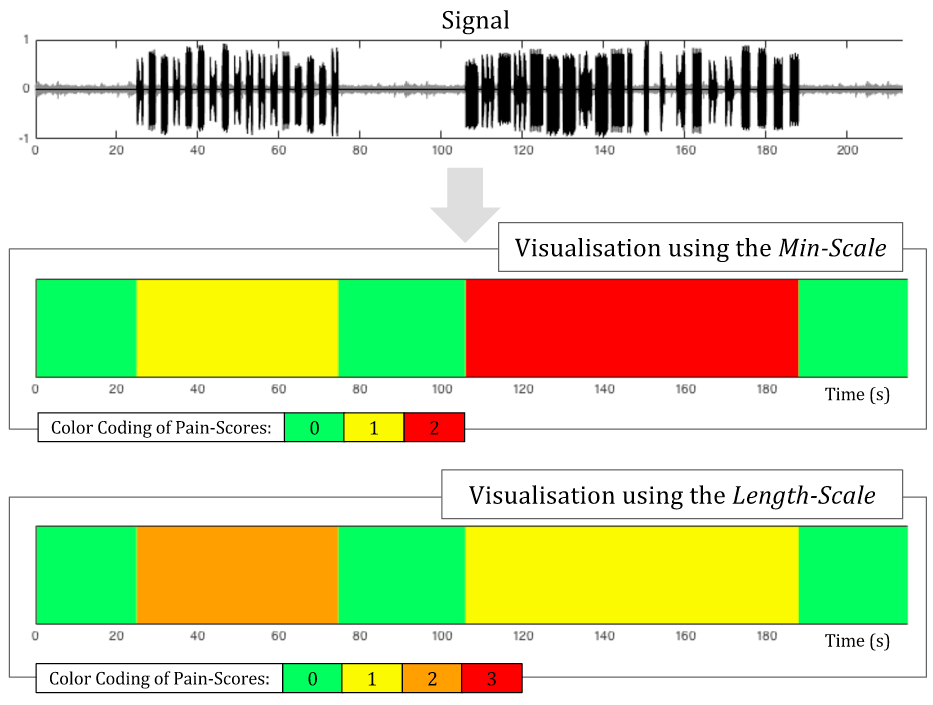
\includegraphics[width=0.85\textwidth]{bilder/viz_without_t_05.png}
	\caption{Visualisierungen der beispielhaften Schmerz-Scales \emph{Length-Scale} und \emph{Min-Scale} für das Beispielsignal. }
	\label{fig:viz_without_t_01}
\end{figure}

Wird das Signal kontinuierlich eingelesen, kann die Einfärbung einer Region mit einem Schrei-Segment erst erfolgen, sobald die Schmerzbewertung durchgeführt wurde und der entsprechende Schmerz-Score feststeht. Die Einfärbung einer Region ohne zugehöriges Schrei-Segment kann hingegen kontinuierlich geschehen, da hier der Schmerz-Score von 0 in jedem Fall feststeht. Würde das Beispielsignal in Abbildung \ref{fig:viz_without_t_01} weiter kontinuierlich eingelesen werden, so würde der Visualisierungsbalken ebenso kontinuierlich fortgesetzt und dabei grün eingefärbt werden. Sobald der Beginn eines neuen Schrei-Segmentes festgestellt wird, kann die dazugehörige, neue in den Balken eingefügte Region erst eingefärbt werden, sobald dieses neue Segment abgeschlossen und die Schmerzbewertung durchgeführt wurde.
 
\section{Visualisierung der Schmerzbewertung mit einander überlappenden Zeitbereichen}
\label{sec:vizResults} 
 
Die Visualisierung von \glqq Zwischenergebnissen\grqq{} bezüglich der Pain Score von Cry-Segmenten lässt sich mit Hilfe des in Kapitel \ref{sec:actulization} vorgestellten Aktualisierungsintervalls $t_{act}$ umsetzen. Die so entstehenden Subsegmente führen zu einander überlappenden Regionen, wie Abbildung \ref{fig:viz_multiple_regions} veranschaulicht. Oben in der Abbildung ist das Beispielsignal zu sehen, welches mit $t_s = \SI{10}{\second}$ segmentiert wurde. Es wurde ein Aktualisierungsintervall von  $t_{act} = \SI{20}{\second}$ und ein Beobachtungszeitraum von $t_{obs} = \infty$ verwendet. Die Aktualisierungszeitpunkte werden durch kleine Pfeile angezeigt. Die letzte Aktualisierung jedes Segmentes wird durch die jeweilige Beendigung eingeleitet. Unten werden die aus den Subsegmenten entstandenen, einander überlappenden Regionen abgebildet. Für jede Region wir der Score angegeben, der sich nach \emph{Min-Scale} ergibt. Die Regionen werden nach dem Schema $L_4$ eingefärbt.

\begin{figure}[h]
	\centering
	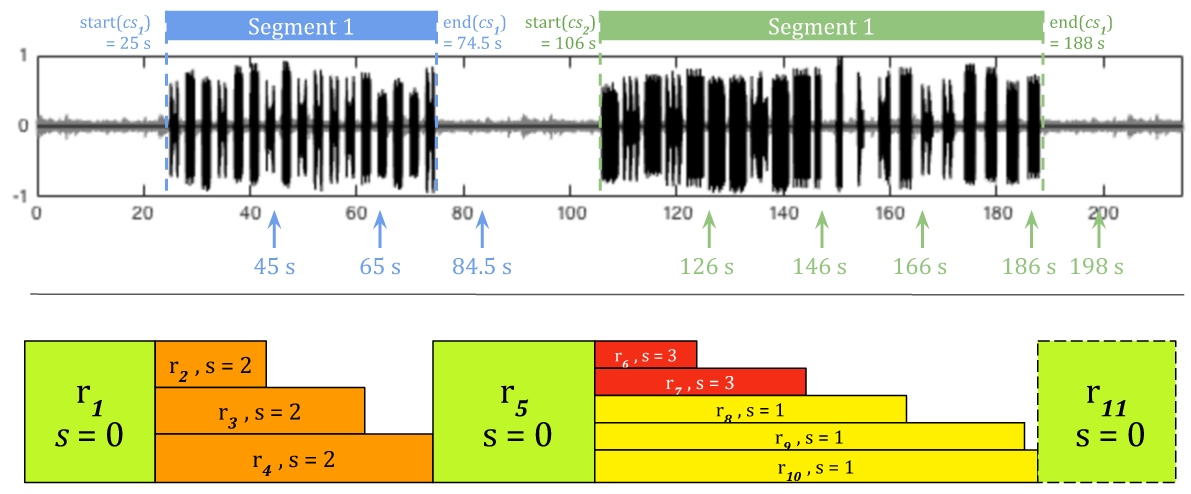
\includegraphics[width=1\textwidth]{bilder/viz-multiple-regions.png}
	\caption{Oben: Beispielsignal mit zwei Segmenten. Unten: Überlappende Regionen, eingefärbt nach dem Farbschema der \emph{Min-Scale}.}
	\label{fig:viz_multiple_regions}
\end{figure}

Es werden zwei Möglichkeiten zur Visualisierung einander überlappender Regionen vorgeschlagen:

\begin{itemize}
\item Die jeweils \glqq aktuellere\grqq{} Region, also diejenige mit dem jeweils \emph{späteren} Endzeitpunkt, überlagert die jeweils \glqq ältere\grqq{} Region, also diejenige mit dem jeweils \emph{früheren} Endzeitpunkt. So wird der jeweils aktuellere Score in den Vordergrund gestellt. Die Historie der abgeleiteten Scores geht jedoch in der Visualisierung verloren. Abbildung \ref{fig:viz_act_over} verdeutlicht dieses Prinzip an einem Beispiel. Das Beispielsignal wurde hier erst bis zu Sekunde $146$ eingelesen, das zweite Segment ist noch geöffnet. Bei der Aktualisierung zum Zeitpunkt $t=\SI{146}{\second}$ wird nach der Min-Scale ein Score von 3 abgeleitet und die Region dementsprechend rot eingefärbt. Das Signal wird nun weiter eingelesen. Bei der nächsten Aktualisierung bei $t=\SI{166}{\second}$ wird ein Score von 1 abgeleitet. Die gelb gefärbte Region überlagert die rot gefärbte Region.

\begin{figure}[h]
	\centering
	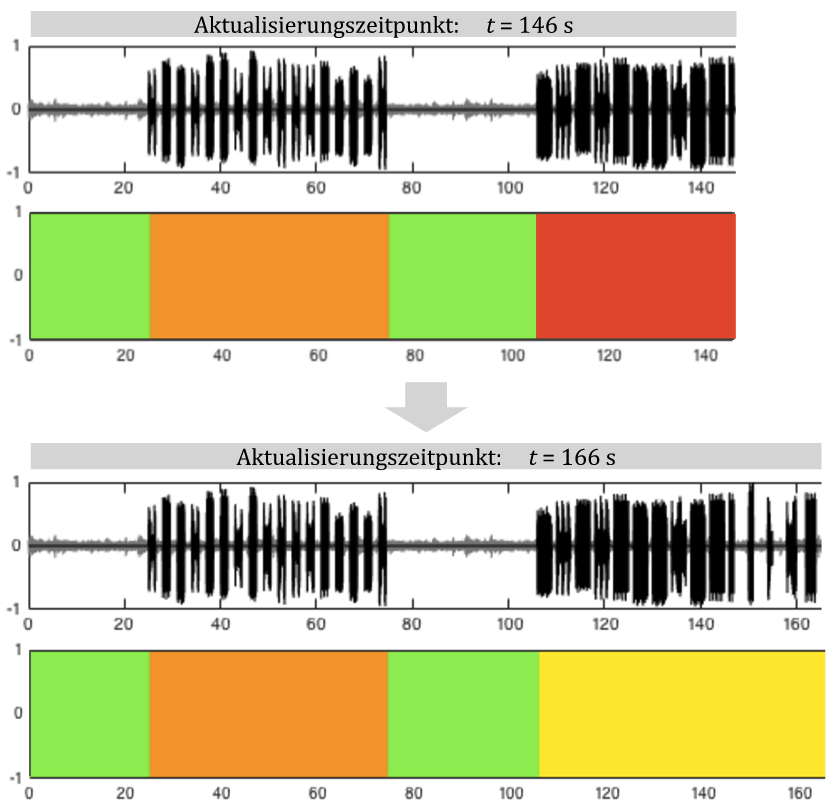
\includegraphics[width=0.7\textwidth]{bilder/viz_act_over_02.png}
	\caption{Visualisierung der Min-Scale bei Aktualisierungen. Die jeweils \glqq aktuellere\grqq{} Region überlagert die jeweils \glqq ältere\grqq{}. Oben: Visualisierung zum Aktualisierungszeitpunkt $t=\SI{146}{\second}$. Unten: Visualisierung zum Aktualisierungszeitpunkt $t=\SI{166}{\second}$.}
	\label{fig:viz_act_over}
\end{figure}

\item Der entgegengesetzte Fall: Die Region mit dem jeweils \emph{früheren} Endzeitpunkt überlagert die Regionen mit dem jeweils \emph{späteren} Endzeitpunkt. So wird die Historie der abgeleiteten Scores in der Visualisierung erkennbar. Abbildung \ref{fig:viz_act_under} zeigt die Visualisierung der Min-Scale für das Beispielsignal nach diesem Prinzip. Wie zu sehen ist, bleibt auch nach Aktualisierung des Scores des zweiten Segmentes auf 1 erkennbar, dass bei früheren Aktualisierungen ein Score von 3 abgeleitet wurde.

\begin{figure}[h]
	\centering
	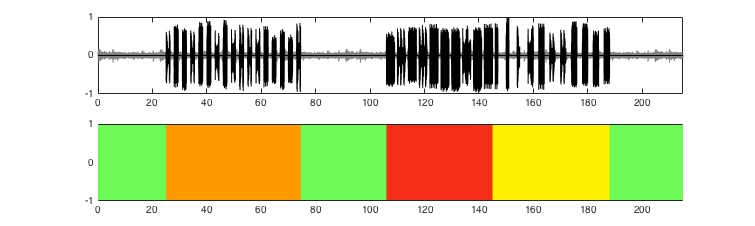
\includegraphics[width=1\textwidth]{bilder/viz_act_under_02.png}
	\caption{Visualisierung der Min-Scale bei Aktualisierungen. Die jeweils \glqq ältere\grqq{} Region überlagert die jeweils \glqq aktuellere\grqq{}.}
	\label{fig:viz_act_under}
\end{figure}
 
\end{itemize}
